
\subsection{Europa}

La instancia elegida para analizar en Europa, fue la universidad Complutense de Madrid (\textit{ucm.es}), ubicada aproximadamente a
5 km de la capital de Madrid. El objetivo de ésta instancia, fue hacer un traceroute a una universidad de Europa central, para poder 
probar y analizar alguna universidad que se situe en Europa y que obligatoriamente tenga que dar el salto del Reino Unido a Europa, 
y así poder observar si hay mucha diferencia o no, en cuanto a tiempos y performance, de ese salto obligatorio de más. \\

Para éste caso, se esperaba que haya tres saltos intercontinentales. Uno de Argentina a USA, otro de USA a Inglaterra (esto lo esperabamos
porque primero hicimos el experimento de analizar una universidad en Inglaterra, no suponiamos ni sabiamos que de Estados Unidos iba a pasar
por Inglaterra) y un último salto de Ingleterra a España. Esto sucede y lo podemos observar gracias a los resultados obtenidos. \\

Los datos de la tabla a continuación, fueron el resultado de 30 iteraciones para cada TTL, hasta la universidad de Madrid: \\


\begin{tabular}{ |p{2cm}||p{3cm}|p{3cm}|p{3cm}|p{3cm}|p{3cm}|   }
 \hline
 \multicolumn{6}{|c|}{Traceroute a Madrid, España} \\
 \hline
 \textit{TTL} & \textit{IP}  & \textit{RTT} & $\delta$\textit{RTT} & \textit{z}$\delta$\textit{RTT}& \textit{Outlier?}\\
 \hline
 1   & Sin respuesta  & - &   - & - & -\\
 2   & 10.10.10.1 & 4.44 ms &   - & - & -\\
 3   & 190.3.128.11  & 16.21 ms & 11.77 ms & 0.94 & - \\
 4   & 190.3.128.34   & 88.34 ms &  72.13 & 0.75 & OUTLIER!\\	
 5   & 64.215.24.153  & 26.15 ms &  - & - & -\\
 6   &  67.17.94.249 & 135.03 ms &  46.69 ms & 0.04 & -\\
 7   & Sin respuesta  & - &  - & - & -\\
 8   & 4.69.210.222  & 241.96 ms & 106.93 ms &  1.73 & OUTLIER!\\
 9   & 4.69.210.222 & 272.3 ms &  30.35 ms & 0.42 & -\\
 10   & 213.242.113.78   & 276.11 ms & 3.8 ms & 1.17 & -\\
 11   & 130.206.245.1   & 243.12 ms & - & - & -\\
 12   & 130.206.212.106  & 244.43 ms &  - & - & -\\
 13   & Sin respuesta  & - & - & - & -\\
 14   & Sin respuesta  & - & - & - & -\\
 15   & Sin respuesta  & - & - & - & -\\
 16   & Sin respuesta  & - & - & - & -\\
 17   & Sin respuesta  & - & - & - & -\\
 18   & Sin respuesta  & - & - & - & -\\
 19   & Sin respuesta  & - & - & - & -\\
 20   & Sin respuesta  & - & - & - & -\\
 21   & Sin respuesta  & - & - & - & -\\
 22   & Sin respuesta  & - & - & - & -\\
 23   & Sin respuesta  & - & - & - & -\\
 24   & Sin respuesta  & - & - & - & -\\
 25   & Sin respuesta  & - & - & - & -\\
 26   & Sin respuesta  & - & - & - & -\\
 27   & Sin respuesta  & - & - & - & -\\
 28   & Sin respuesta  & - & - & - & -\\
 29   & Sin respuesta  & - & - & - & -\\
 30   & Sin respuesta  & - & - & - & -\\
 31   & Sin respuesta  & - & - & - & -\\
 \hline
\end{tabular} \\ \\


Análisis de la tabla de RTT's: \\ \\

La primera respuesta que obtenemos es para TTL=1, la IP 10.10.10.1 se corresponde con el router Wi-Fi que se está utilizando en el hogar del 
integrante que corrió el experimento. Se corresponde con una red privada que no es visible para afuera y que utiliza protocolo IP versión 4 (IPv4). \\ \\

Las IP's de TTL=3 y TTL=4 se corresponden con las IP's de la Cooperativa Telefonica de Telviso, proveedor de internet ubicado en 
la localidad de Del Viso, partido de Pilar (zona norte GBA). \\ \\

La IP de TTL=5 se corresponde con un servidor ubicado en Capital Federal, llamado Level 3 Communications Inc. Esta empresa es una 
compañía multinacional estadounidense de telecomunicaciones y proovedor de servicios de Internet radicado en Broomfield, Colorado. A eso se debe que  
después de este salto, el paquete de IP va hacia Estados Unidos.  \\ \\

Para el TTL=6 se encontró que la IP se corresponde con un servidor en la ciudad de Wichita, perteneciente al estado de Kansas, EEUU. 
Esto se dedujo buscando la ip en internet. En la página http://myip.es\\ \\

Para los TTL=8 y TTL=9 la IP se corresponde todavía en territorio de los Estados Unidos. \\ \\

Luego, la IP 213.242.113.78 se ubica en un servidor de Londres, Inglaterra. A eso se debe la gran diferencia que se puede observar en el 
gráfico de Saltos vs RTT's del desvío standart. \\ \\

La IP 130.206.245.1 con TTL=11 se ubica en la ciudad de Madrid, España. Este es el tercer salto intercontinental que se observa 
(los dos anteriores eran de Argentina a Estados Unidos y de este último a Londres). \\ \\

La última IP se encuentra en Valencia, España. Si bien la Universidad Complutense de Madrid se ubica precisamente en Madrid, 
puede pasar que el servidor que almacena la url de la universidad se encuentre en otro lugar, esto se puede deber a costos o cuestiones logisticas.\\ \\ \\


Conclusiones: \\ \\

El primer salto intercontinental es del TTL=6, de Argentina a Estados Unidos. Esto se puede observar en la diferencia de mili segundos entre 
el RTT de la IP 64.215.24.153 y la IP 67.17.94.249, ya que el primero tarda un promedio de 26.15 ms en responder y el segundo tarda 135.03 ms,
una diferencia considerable. \\ \\

El TTL=8 tiene 106.93 ms de diferencia con respecto al anterior y además cambia de IP. Al tener un RTT muy alto con respecto al anterior,
podemos llegar a suponer que el paquete podría llegar a estar en una ciudad costera de Estados Unidos, para después poder dar el salto a Inglaterra,
ya que salte directo de Colorado o Kansas hasta Inglaterra no tendría mucho sentido. \\ \\

El segundo salto intercontinental es el de la IP 213.242.113.78 . Esto se puede deducir gracias al gráfico saltos vs RTT's, que muestra como pega un
salto la función roja que mide el zRTT, en el gráfico 'saltos vs dRTTs'.\\ \\

El tercer salto intercontinental es de la IP 130.206.245.1 donde se puede apreciar una diferencia en el gráfico de barras 
(saltos vs RTTs) con respecto a la IP anterior (213.242.113.78), si bien es un enlace subacuático,
las distancias no son demasiado extensas como para que haya una diferencia muy grande en cuanto a tiempos. \\ \\

Para TTL >= 13 no hay respuestas porque bastaron con 12 saltos (hops) para llegar a la ip de la Universidad de Madrid. Por ese motivo, 
no hay respuestas para esos casos. \\ \\ 


El porcentaje de saltos que no responden los Time exceeded es: 21 paquetes con cierto TTL que no responden / 31 TTLs distintos = 0.68\%.  \\ \\


En total para esta instancia, se encontraron 2 outliers posibles según el método de Cimbala. Uno es del TTL=4 y el otro para el TTL=8. 
Estos outliers son con respecto a la diferencia entre el RTT actual y el RTT anterior, en valores de mili segundos.\\ \\


Según lo que se pudo averiguar y las conclusiones a las que se llegó, ninguno de los dos outliers se corresponden con enlaces intercontinentales 
y subacuáticos. El primer outlier (para el TTL=4) se corresponde con el proveedor de internet del hogar donde se ejecutó el programa.
Y el segundo outlier, por lo que se analizó, se debe a la gran distancia entre la IP del servidor del estado de Kansas (centro de USA) 
y el servidor de alguna ciudad costera de Estados Unidos. Por lo tanto, se obtuvieron dos falsos negativos, en cuanto a los outliers obtenidos. \\ \\










\pagebreak


\begin{figure}[!h]
\centering
\caption{Saltos vs RTT}
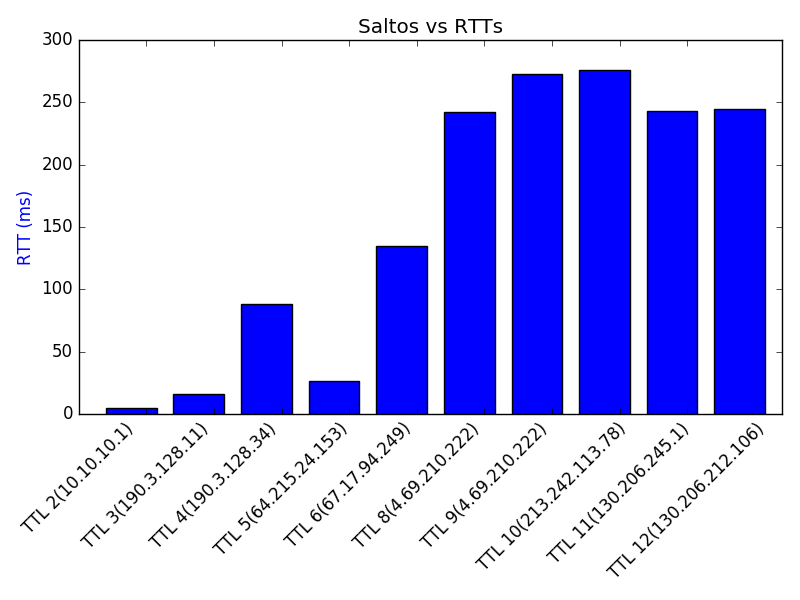
\includegraphics[width=0.75\textwidth]{modules/EU-saltos-rtt}
\label{fig:EU-saltos-rtt}
\end{figure}


\begin{figure}[!h]
\centering
\caption{Saltos vs dRTT}
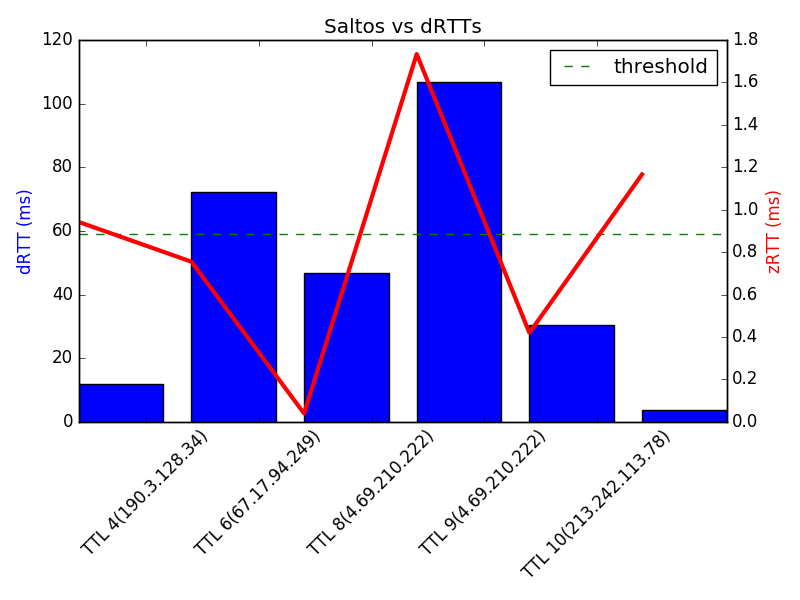
\includegraphics[width=0.75\textwidth]{modules/EU-saltos-drtt}
\label{fig:EU-saltos-drtt}
\end{figure}


\pagebreak

\begin{figure}[!h]
\centering
\caption{traceroute de ARG a ESP}
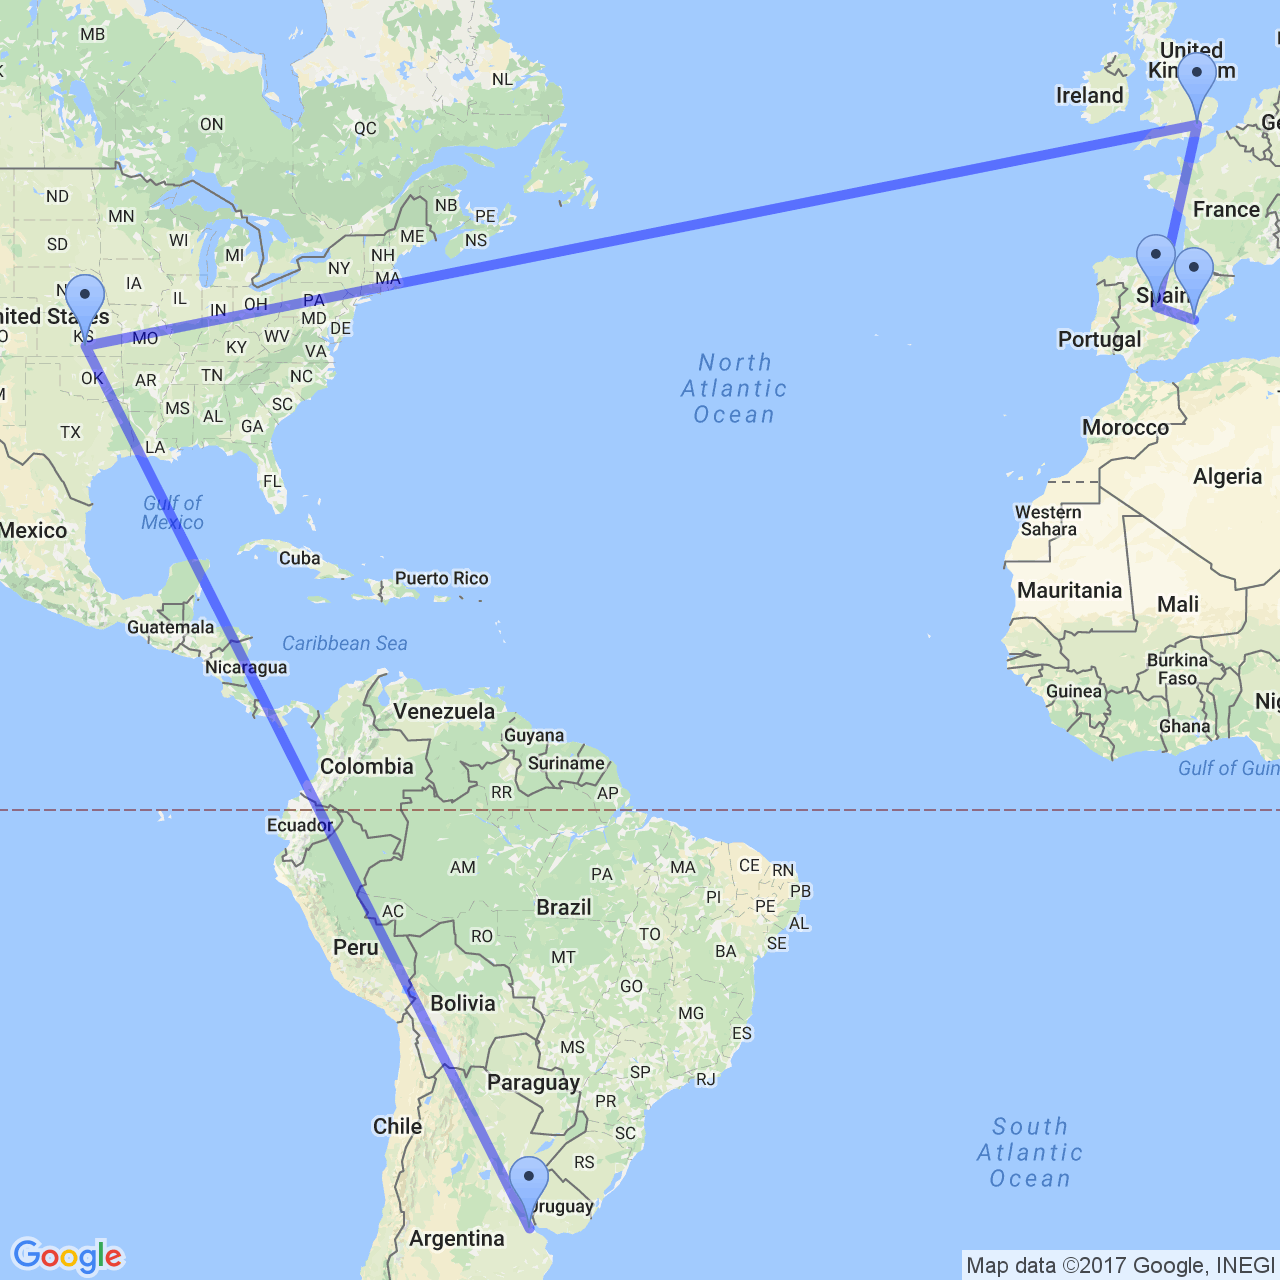
\includegraphics[width=0.75\textwidth]{modules/traceroute-EU}
 \label{fig:traceroute-EU}
\end{figure}
